\newpage
\bignumberedpart{Моделювання}

\subsection{Практичний доказ}
\label{poc}
Для доказу роботи та дослідження роботи алгоритму був написаний прототип (proof of concept) \cite{rader2014cdr}. Алгоритм \ref{alg:general_anomaly_detection} реалізований без змін мовою Python. Візуалізація шаблонів двох класів користувачів на \autoref{fig:model_poc_1}. Перший клас - абоненти, що роблять дзвінки на початку і в кінці робочого дня, а також активні у вихідні дні. Другий клас - типово корпоративні користувачі, що роблять дзвінки в бізнес-години. Як видно, вноситься випадкова складова по днях тижня, і для кожного абонента вона своя.

У імітаторі є можливість провести інтервенцію однієї групи користувачів, або декількох, переводячи з одного сталого стану в інший. Таким чином є можливість протестувати роботу системи виявлення аномальної поведінки.

\begin{figure}[h]
        \begin{center}
            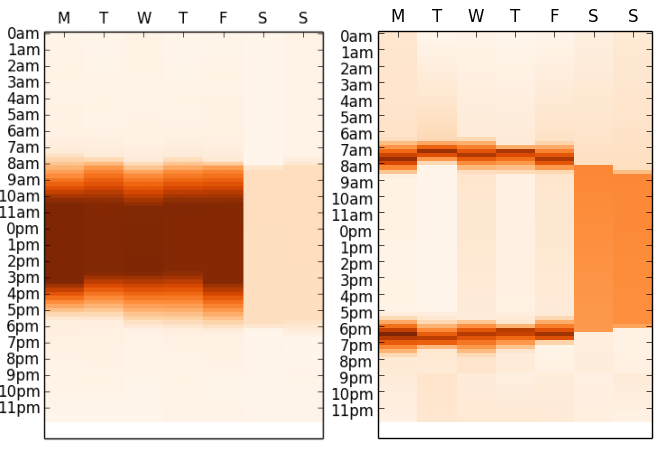
\includegraphics[scale=0.4]{resources/model_1_2.png}
        \end{center}
        \caption{Два класи імітованих абонентів}
        \label{fig:model_poc_1}
\end{figure}

Проаналізовано роботу алгоритму в трьох випадках:
\begin{itemize}
  \item Інтервенція в роботу тільки одного абонента (\autoref{fig:model_poc_one});
  \item Інтервенція в роботу одного класу абонентів, робота без урахування тренда (\autoref{fig:model_poc_group_notrend}). По осі абсцис - час у годинах (в моделі) з початку роботи системи, по осі ординат - кількість дзвінків;
  \item Інтервенція в роботу одного класу абонентів, робота з урахуванням тренда (\autoref{fig:model_poc_group}).
\end{itemize}


\begin{figure}[h!]
        \begin{center}
            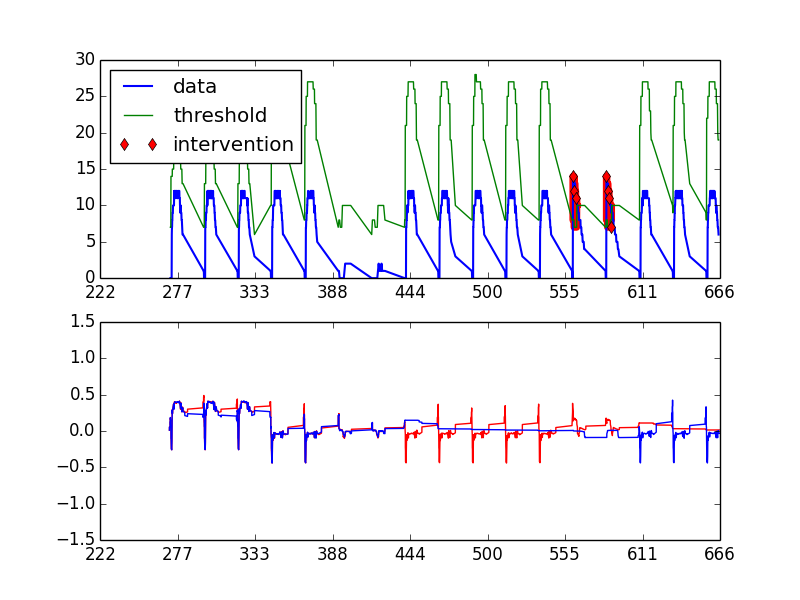
\includegraphics[scale=0.6]{resources/model_1_3_one.png}
        \end{center}
        \caption{Одинична інтервенція одного телефонного номера у вихідні дні. По осі абсцис - час у годинах (в моделі) з початку роботи системи, по осі ординат - кількість дзвінків}
        \label{fig:model_poc_one}
\end{figure}

\begin{figure}[h!]
        \begin{center}
            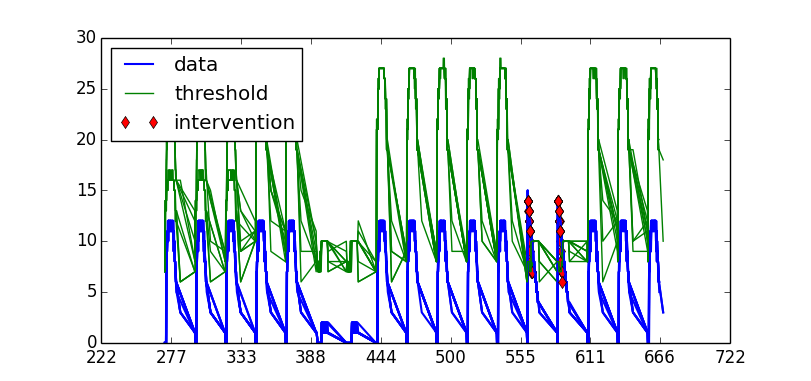
\includegraphics[scale=0.6]{resources/model_1_4_group_notrend.png}
        \end{center}
        \caption{Інтервенція в роботу одного класу абонентів без урахування тренда}
        \label{fig:model_poc_group_notrend}
\end{figure}

\begin{figure}[h!]
        \begin{center}
            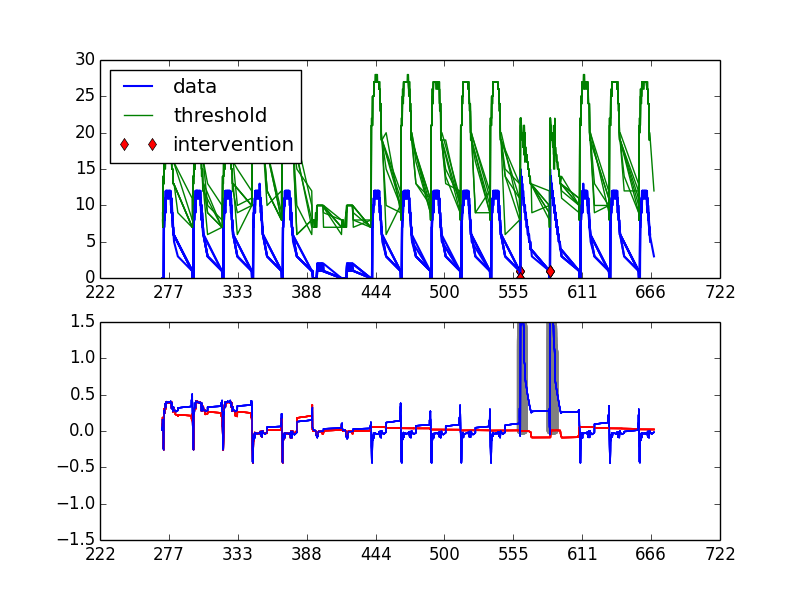
\includegraphics[scale=0.6]{resources/model_1_5_group.png}
        \end{center}
        \caption{Інтервенція в роботу класу абонентів з урахуванням тренда}
        \label{fig:model_poc_group}
\end{figure}


На верхніх графіках показана залежність кількості дзвінків, максимально допустиму кількість дзвінків і точками позначені виявлені інтервенції. На нижніх графіках показаний тренд.

Як видно, при інтервенції в роботу одного абонента (\autoref{fig:model_poc_one}) тренд не змінюється і інтервенція виявляється легко (кількість підозрілих дзвінків практично збігається з фактичною).

При груповій зміні поведінки (\autoref{fig:model_poc_group}) видно два піки лінії тренда, що припадають на вихідні дні (в даному досліді користувачі, які ніколи не дзвонили по вихідних змінюють цю поведінку). На верхньому графіку видно, що рівень інтервенцій дуже низький, що означає правильну роботу алгоритму - групова зміна поведінка не вважається підозрілим.

Для перевірки, другий дослід був проведений з тими ж вихідними даними, але без урахування тренда (\autoref{fig:model_poc_group_notrend}). На графіку видно, що рівень інтервенцій практично збігається з кількістю фактичних дзвінків в даній ділянці, що значить високу ймовірність шахрайства. Таким чином, спосіб обліку групових змін дійсно зменшує кількість помилкових спрацьовувань.

Як видно з \autoref{fig:model_poc_time}, час обробки одного запису не є константним. Ця характеристика стає гіршою із збільшенням кількості абонентів.

\begin{figure}[h!]
        \begin{center}
            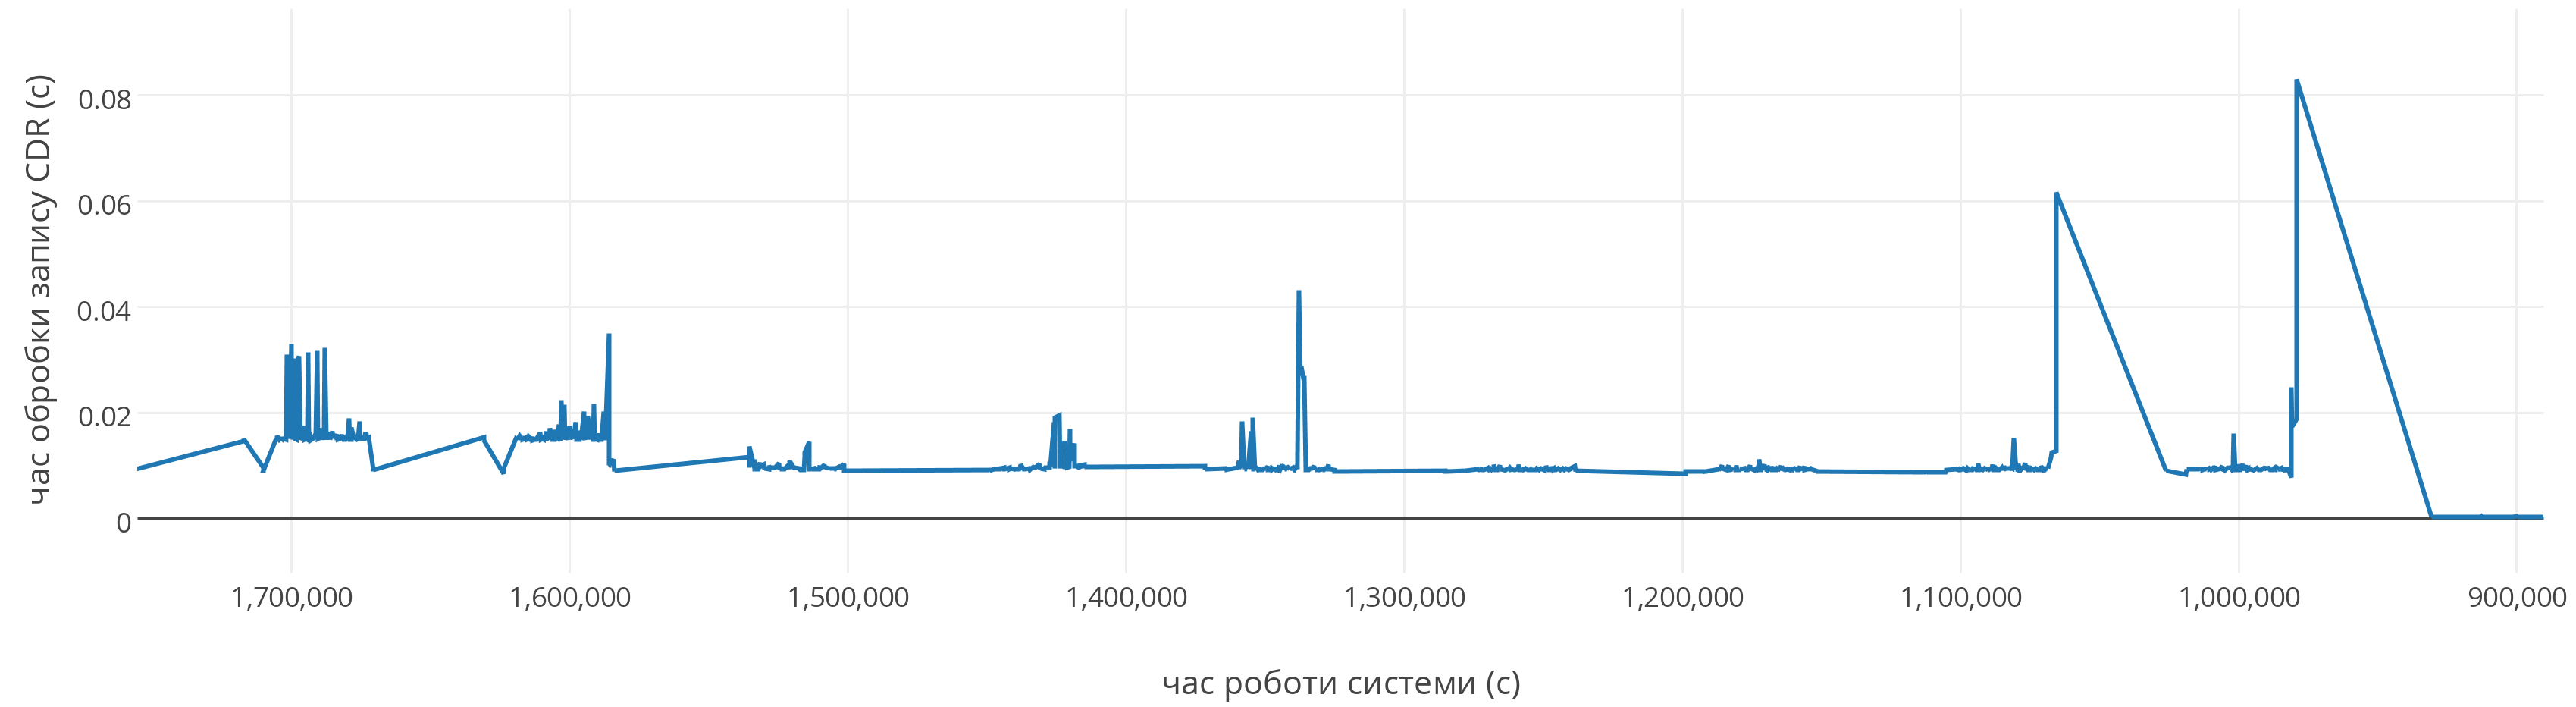
\includegraphics[scale=0.15]{resources/poc-time.png}
        \end{center}
        \caption{Час обробки записів у прототипі системи}
        \label{fig:model_poc_time}
\end{figure}

\subsection{Реалізація алгоритму після модифікації}

Для усунення недоліків вихідного алгоритму, він був декомпозований для роботи в паралельному режимі (розділ \ref{parallel}).

Імітатор налаштований для роботи з двома класами абонентів (\autoref{fig:model_prod_1}).

\begin{figure}[h!]
        \begin{center}
            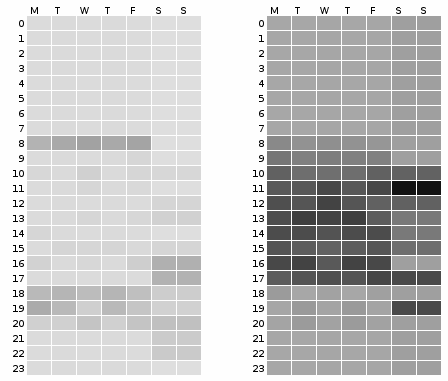
\includegraphics[scale=0.6]{resources/model_2_1.png}
        \end{center}
        \caption{Два класи імітованих абонентів}
        \label{fig:model_prod_1}
\end{figure}

В результаті класифікації кожен абонент потрапляє в одну з k груп (На \autoref{fig:model_prod_2} позначені кольорами та цифрою зверху справа).

\begin{figure}[h!]
        \begin{center}
            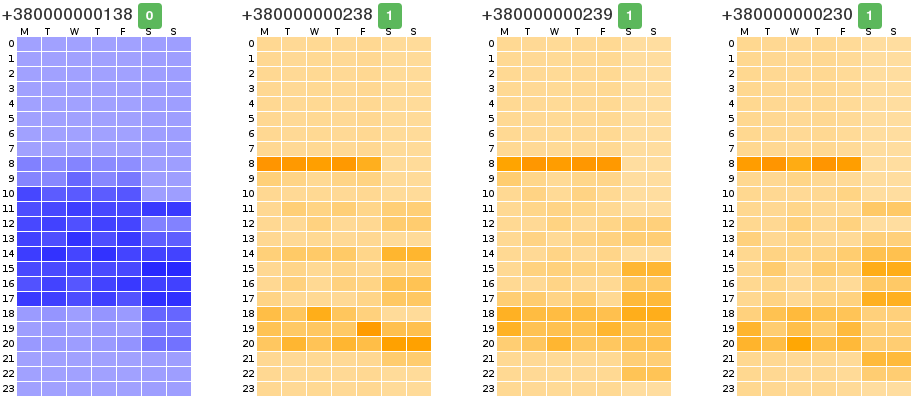
\includegraphics[scale=0.4]{resources/model_2_2.png}
        \end{center}
        \caption{Результат класифікації абонентів}
        \label{fig:model_prod_2}
\end{figure}

Як видно з порівняння \autoref{fig:model_prod_time} та \autoref{fig:model_poc_time}, у розробленій системі враховані недоліки першої реалізації, час обробки одного запису зменшився на 50\%, при чому в новій реалізації характеристика не залежить від кількості абонентів чи класів.

\begin{figure}[h!]
        \begin{center}
            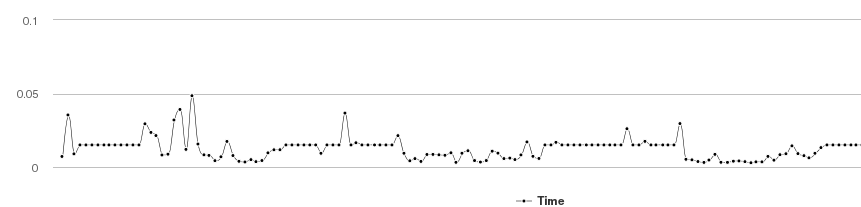
\includegraphics[scale=0.5]{resources/system-time.png}
        \end{center}
        \caption{Час обробки записів у розробленій системи}
        \label{fig:model_prod_time}
\end{figure}

\subsection{Моделювання за відсутності інтервенцій}

Після моделювання 100 абонентів, по 50 абонентів на один шаблон поведінки, отримані такі дані. На \autoref{fig:model_prod_3} зображено графік аналізу одного із абонентів мережі. Як видно з графіку, реальне використання абонентом мережі (суцільна лінія) близька до розрахованого шаблону поведінки (пунктирна лінія), та лежить в межах довірчого інтервалу 95\% (сіра зона на графіку).

\begin{figure}[h!]
        \begin{center}
            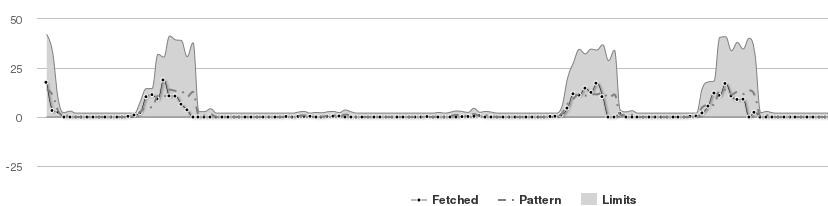
\includegraphics[scale=0.55]{resources/model_2_3.png}
        \end{center}
        \caption{Графік аналізу роботи одного з абонентів}
        \label{fig:model_prod_3}
\end{figure}

Відхилення частоти використання мережі абоненту від шаблонної (\autoref{fig:model_prod_4}) в межах допустимих границь.

\begin{figure}[h!]
        \begin{center}
            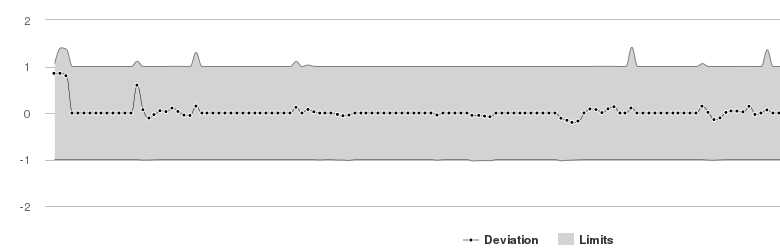
\includegraphics[scale=0.55]{resources/model_2_4.png}
        \end{center}
        \caption{Графік відхилення частоти дзвінків одного з абонентів від шаблону}
        \label{fig:model_prod_4}
\end{figure}

За відсутності змін поведінки, тренд (\autoref{fig:model_prod_5}) флуктує біля позначки 0.

\begin{figure}[h!]
        \begin{center}
            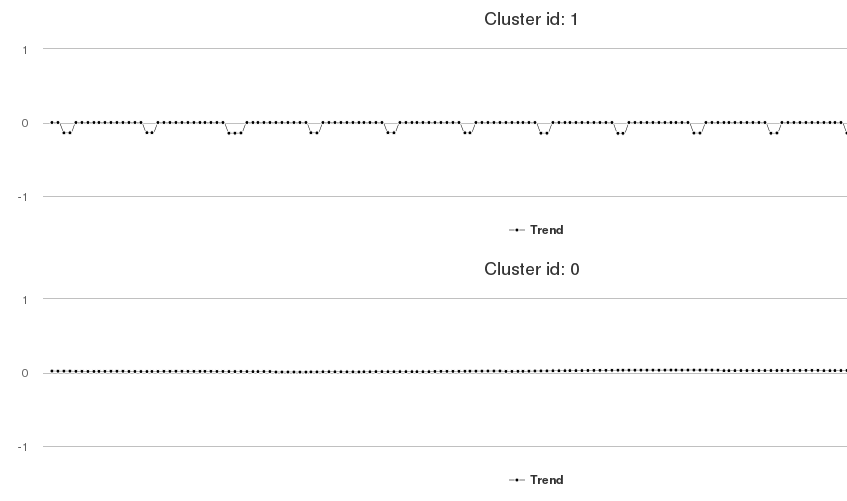
\includegraphics[scale=0.55]{resources/model_2_5.png}
        \end{center}
        \caption{Графік тренду, розрахованого для двох кластерів}
        \label{fig:model_prod_5}
\end{figure}

% график времени обработки (должна быть константа), типа круто же

\subsection{Результати моделювання для алгоритму без урахування тренду}
    \TBD
\subsection{Результати моделювання для алгоритму з урахуванням тренду}
    \TBD
% \newpage
\subsection*{Висновки до розділу 3}
\addcontentsline{toc}{subsection}{Висновки до розділу 3}

Було промодельовано розроблений прототип системи виявлення аномалій поведінки абонентів телефонної мережі. На базі моделювання були виявлені недоліки та розроблені вимоги до системи. Промодельовано роботу розробленої системи та зроблено порівняння із прототипом.

Проаналізовано роботу алгоритму в багатокористувацькому режимі з урахуванням тренда, а також проведено порівняння з однокористувацьким режимом і багатокористувацьким режимом без урахування тренда режимах для оцінки ефективності методу.

Як видно з результатів моделювання, розроблена система, на відміну від її прототипу, видає константний час на перевірку одного номеру, що дозволяє використовувати систему із обмеженнями реального часу.
